\objectives{%
  \item define (in both math and code) a class of linear hypotheses for given featurized data
  \item compute the perceptron and hinge losses a given hypothesis suffers
        on given data
}

% -- what hypotheses will we consider?  a recipe for $\hH$
% -- how good is a hypothesis?  fit
% -- which hypothesis is best?  optimization by gradient descent
% -- how good is a hypothesis?  plausibility
% -- two more tasks
% -- improving approximation, optimization, generalization

\sampassage{what hypotheses will we consider?  a recipe for $\hH$}
  Remember: we want our machine to find an input-to-output rule.  We call
  such rules \textbf{hypotheses}.  As engineers, we carve out a menu $\hH$ of
  rules for the machine to choose from.
  %
  We'll consider
  hypotheses of this format:
  \emph{extract features} of the input to make a list of numbers; then
  \emph{linearly combine} those numbers to make another list of numbers;
  finally,
  \emph{read out} a prediction %a distribution over output values
  from the latter list.
  Our digit classifying hypotheses, for instance, look like:\bovinenote{%
    Our list \texttt{threeness} has length one: it's just a fancy way of talking
    about a single number.  We'll later use longer lists to model richer outputs:
    to classify between $>2$ labels,
    to generate a whole image instead of a class label, etc.
    The concept of \texttt{threeness} (and what plays the same role in other
    ML projects) is called the \textbf{decision function}.  The decision function
    takes an input $x$ and returns some kind of score for what the final
    output should be.  The decision
    function value is what we feed into the readout.
  }
  \begin{lstlisting}[language=Python, basicstyle=\footnotesize\ttfamily]
    def predict(x):
      features = [brightness(x), width(x)]              # featurize
      threeness = [ -1.*features[0] +4.*features[1] ]   # linearly combine
      prediction = 3 if threeness[0]>0. else 1          # read out prediction
      return prediction
  \end{lstlisting}
  The various hypotheses differ only in those coefficients (jargon:
  \textbf{weights}, here $-1, +4$) for their linear combinations; it is these
  degrees of freedom that the machine \emph{learns} from data.
  %
  %We can diagram such hypotheses by drawing arrows:
  These arrows summarize the situation:\bovinenote{%
      This triple of arrows is standard in ML.  But the name
      `readout' is not standard jargon.  I don't know standard jargon for this
      arrow.
  }
  \[
    \xX   \xrightarrow[\text{\color{gray}not learned}]{\text{featurize}}
    \Rr^2 \xrightarrow[\text{\textbf{learned!}}]{\text{linearly combine}}
    \Rr^1 \xrightarrow[\text{\color{gray}not learned}]{\text{read out}}
    \yY
    %\text{DistributionsOn}(\yY)
  \]
  %
  Our Unit 1 motto is to \emph{learn a linear map flanked by hand-coded
  nonlinearities}.  We design the nonlinearities to capture domain knowledge
  about our data and goals.

  \begin{figure}[h]
    \centering%
    \picturew{0.85\textwidth}{beach.png}%
    \caption{%
      \textbf{The \emph{slope} of the decision function's graph is meaningful,
      even though it doesn't affect the decision boundary.}
      We plot the decision function (vertical axis) over
      weight-space (horizontal axes) (\textbf{black dot}).  The graph is an infinite plane, a
      hexagonal portion of which we show; it attains zero altitude
      at the {\dgre decision boundary}.
      We interpret high (low)
      altitude as `confident the label is {\rng orange} ({\blu blue})';
      intermediate altitudes, as leaning but without confidence.
      %
      We'll introduce a notion of `goodness-of-fit-to-data'
      that seeks not just to correctly classify all the training points BUT
      ALSO to do so with confidence.  That is, we want {\rng orange} ({\blu
      blue}) training points to all be above (below) the {\dgre gray `shelf'}
      that delimits high-confidence.
      %
      I like to imagine a shoreline: an interface between
      {\blu{water}} and {\rng{beach}}.  We want to adjust the topography so
      that all {\blu blue} ({\rng orange}) training points are deep underwater (high and dry).
    \attnsam{caption}
    }
  \end{figure}

  %\attnsam{CONFIDENCE}

  For now, we'll assume we've already decided on our featurization and we'll
  use the same readout as in the
  code above:\bovinenote{%
    \attnsam{paragraph flow?!} 
    Intuitively, \texttt{threeness} is the machine's \textbf{confidence} that the answer
    is ${\rng 3}$.  Our current readout discards all information except for the
    sign: we forget whether the machine was very confident or slightly confident
    that the answer is ${\rng 3}$, so long as it prefers ${\rng 3}$ over ${\blu
    1}$.  However, we will care about confidence levels when assessing
    goodness-of-fit.
  }
  \begin{lstlisting}[language=Python, basicstyle=\footnotesize\ttfamily]
  prediction = 3 if threeness[0]>0. else 1          # for a digit-classifying project
  prediction = 'cow' if bovinity[0]>0. else 'dog'   # for an animal-classifying project
  \end{lstlisting}
  That's how we make predictions from those ``\textbf{decision function values}''
  \texttt{threeness} or \texttt{bovinity}.  But to compute those values we
  need to determine some weights.
  %We'll do so by optimizing some notion of
  %goodness-of-fit.
  \emph{How shall we determine our weights and hence our hypothesis?}
  %by which we'll compute \texttt{threeness} or
  %\texttt{bovinity} from our features?}.

  %Since we select a hypothesis with high goodness-of-fit,


  %if \texttt{threeness} the machine predicts ${\rng 3}; otherwise
  %it predicts ${\blu 1}
  %Of course, if we are classifying dogs vs cows that line would read
  %\begin{lstlisting}[language=Python, basicstyle=\footnotesize\ttfamily]
  %\end{lstlisting}
  %$$
  %  \texttt{cow if bovinity[0]>0.\ else dog}
  %$$


%\newpage
\sampassage{how good is a hypothesis?  fit}
  We instruct our machine to find within our menu $\hH$ a hypothesis that's as
  ``good'' as possible.  That is, the hypothesis should both fit our training
  data and seem intrinsically plausible.  We want to quantify these notions of
  goodness-of-fit and intrinsic-plausibility.  As with $\hH$, how we quantify
  these notions is an engineering art informed by domain knowledge.  Still,
  there are patterns and principles --- we will study two specific quantitative
  notions, the \textbf{perceptron loss} and \textbf{SVM loss}, to study these
  principles.
  %
  Later, once we understand these notions as quantifying uncertainty (i.e., as
  probabilistic notions), we'll appreciate their logic.  But for now we'll
  bravely venture forth, ad hoc!

  We start with goodness-of-fit.  Hypotheses correspond\bovinenote{%
    A very careful reader might ask: \emph{can't multiple choices of weights
    determine the same hypothesis?}  E.g.\ $(-1, +4)$ and $(-10, +40)$ classify every input
    the same way, since they either both make \texttt{threeness} positive or
    both make \texttt{threeness} negative.
    %
    This is a very good point, dear reader, but at this stage in the course,
    much too pedantic!  Ask again later.
  } to
  weights.  For example, the weight vector $(-1, +4)$ determines the
  hypothesis listed above.

  One way to quantify $h$'s goodness-of-fit to a training example $(x,y)$ is to
  see whether or not $h$ correctly predicts $y$ from $x$.  That is, we could
  quantify goodness-of-fit by \emph{training accuracy}, like we did in the
  previous digits example:
  \begin{lstlisting}[language=Python, basicstyle=\footnotesize\ttfamily]
    def is_correct(x,y,a,b):
      threeness = a*brightness(x) + b*width(x)
      prediction = 3 if threeness>0. else 1
      return 1. if prediction==y else 0.
  \end{lstlisting}
  By historical convention we actually like\bovinenote{%
    ML can be a glass half-empty kind of subject!
  }
  to minimize badness (jargon: \textbf{loss}) rather than
  maximize goodness.  So we'll rewrite the above in terms of mistakes:\bovinenote{%
    We'll refer to the ``leeway before a mistake'' throughout this section;
    it's a standard concept but \textbf{not} a concept with a standard name afaik.
  }
  \begin{lstlisting}[language=Python, basicstyle=\footnotesize\ttfamily]
    def leeway_before_mistake(x,y,a,b):
      threeness = a*brightness(x) + b*width(x)
      return +threeness if y==3 else -threeness
    def is_mistake(x,y,a,b):
      return 0. leeway_before_mistake(x,y,a,b)>0. else 1.
  \end{lstlisting}

  We \emph{could} define goodness-of-fit as training accuracy.  But we'll enjoy
  better generalization and easier optimization by allowing ``partial credit''
  for borderline predictions.
  %
  E.g.\ we could use \texttt{leeway\_before\_mistake} as goodness-of-fit:\bovinenote{%
  to define \emph{loss}, we flip signs, hence the `$1-$'
  \exercise{%
    For incentives to point the right way, loss should
    \emph{decrease as \texttt{threeness} increases when \texttt{y==3}} but should
    \emph{increase as \texttt{threeness} increases when \texttt{y==1}}.
    Verify these relations for the several loss functions we define.
  }
  }
  \begin{lstlisting}[language=Python, basicstyle=\footnotesize\ttfamily]
    def linear_loss(x,y,a,b):
      return 1 - leeway_before_mistake(x,y,a,b)
  \end{lstlisting}
  %Notice that if the \texttt{leeway} is very positive, then the badness is
  %very negative (i.e., we are in a very good situation), and vice versa.

  \begin{figure}[h]
    \centering%
    \picturew{0.85\textwidth}{hinge-beach.png}%
    \caption{%
      \textbf{Geometry of leeways, margins, and hinge loss}.
      As before, we graph the decision function (vertical axis) against
      weight-space.  The $y={\blu -1}$ ($y={\rng +1}$) training points $(x,y)$
      sit one unit below (above) the zero-altitude plane.  We draw regions where
      the graph surpasses $\pm 1$ altitude as {\dgre shaded
      `shelves'}.
      %
      %%Though `down' means {\blu blue}, a point can lie below the graph yet
      %%be classified as {\rng orange} --- see the rightmost training points.
      %
      \textbf{Leeway} is the vertical distance between a {\gre gray} $x$
      and the graph (and it's positive when the point is correctly classified).
      %
      \textbf{Linear loss} is the vertical distance between an $(x,y)$ point
      and the graph (positive when the point is on the `wrong' side of the
      graph, i.e., when the graph lies between the point and the zero-altitude
      plane).
      %
      \textbf{Hinge loss} is linear loss, except no reward is given for any
      distance beyond the `shelves' at $\pm 1$ altitude.  We draw hinge loss
      in \textbf{black vertical segments}.
      %
      A hypothesis's \textbf{margin} is the horizontal distance the edge of
      those `shelves' and the decision boundary.
      %
    \attnsam{caption}
    }
  \end{figure}

  But, continuing the theme of pessimism, we usually feel that a ``very safely
  classified'' point (very positive \texttt{leeway}) shouldn't make up for a
  bunch of ``slightly misclassified'' points (slightly negative
  \texttt{leeway}).\bovinenote{%
    That is,
    %The practical consequence appears during trade-offs:
    we'd rather have \texttt{leeway}s $+.1, +.1, +.1, +.1$
    than $+10, -1, -1, -1$ on four training examples.
    A very positive \texttt{leeway} feels mildly pleasant to us while a
    very negative one feels urgently alarming.
    \exercise compute and compare the training accuracies in these two
    situations.
    %
    %
    As an open-ended followup, suggest reasons why optimizing
    \texttt{leeway}s instead of just accuracies might help
    improve testing accuracy.
  }
  But total linear loss
  %incentivizes the opposite choice:
  doesn't capture this asymmetry;
  %
  to address this, let's impose a floor on
  \texttt{linear\_loss} so that it can't get too negative
  (%To cap \texttt{linear\_loss} from below is to
  i.e., so that
    %cap from above how much we care about \texttt{leeway}:
    positive \texttt{leeway} doesn't count arbitrarily much).
    %
    %It's good to get used to this mental flipping between maximizing goodness
    %and minimizing loss.
  We get \textbf{perceptron loss} if we set a floor of $1$; \textbf{SVM loss}
  (also known as \textbf{hinge loss}) if we set a floor of $0$:
  \begin{lstlisting}[language=Python, basicstyle=\footnotesize\ttfamily]
    def perceptron_loss(x,y,a,b):
      return max(1, 1 - leeway_before_mistake(x,y,a,b))
    def svm_loss(x,y,a,b):
      return max(0, 1 - leeway_before_mistake(x,y,a,b))
  \end{lstlisting}

  %\begin{marginfigure}[-0cm]
  %  \centering
  %  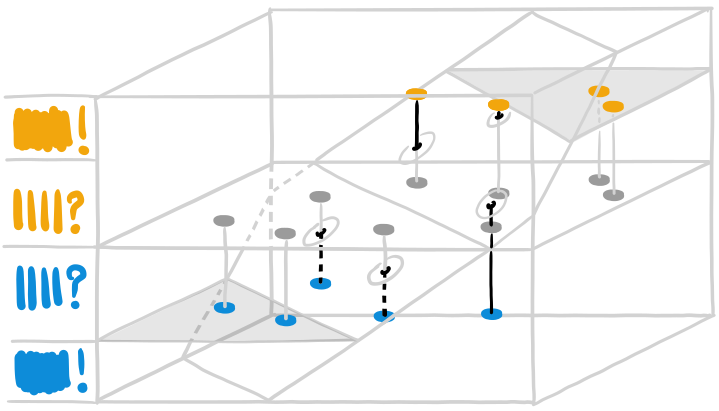
\includegraphics[width=0.99\textwidth]{./hinge-beach.png}
  %  \caption{%
  %  \attnsam{caption}
  %  }
  %\end{marginfigure}



  Proportional weights have the same accuracies but different hinge losses.
  \exercise{Can we say the same of perceptron loss?}
  \begin{figure}[h]
    \centering
    \picturedw{0.23\textwidth}{example-mnist/train-features-hinge-wide-crop.png}%
    \hspace{0.22cm}%
    \picturedw{0.23\textwidth}{example-mnist/train-features-hinge-narrow-crop.png}%
    \hspace{0.22cm}%
    \picturedw{0.46\textwidth}{example-mnist/train-weights-Hinge}
    \caption{%
          \textbf{Hinge loss's optimization landscape reflects confidence, unlike
          training accuracy's.}
          %
          --- \textbf{Left rectangular panes}.  An under-confident and
          over-confident hypothesis.  These have weights
          $(a/3, b/3)$ and $(3a, 3b)$, where
          $(a,b)=(-3.75,16.25)$ minimizes training hinge loss.  The glowing
          colors' width indicates how rapidly \texttt{leeway} changes as we
          move farther from the boundary.
          %
          --- \textbf{Right shaded box}.  The $(a,b)$ plane, centered at the
          origin and shaded by hinge loss, with training optimum {\blu blue}.
          %
          Indecisive $h$s (e.g.\ if
          \texttt{threeness}$\approx 0$) suffer, since $\text{max}(0,1-\ell)\approx
          1$, (not $0$) when $\ell\approx 0$.
          %
          Hinge loss penalizes \emph{overconfident} mistakes severely (e.g.\
          when $y={\blu 1}$ yet \texttt{threeness} is huge):
          $\text{max}(0,1-\ell)$ is unbounded in $\ell$.
          %grows as $\ell$ becomes more negative.
          %
          If we start at the origin $(a,b)=(0,0)$ and shoot (to less
          underconfidence) toward the optimal hypothesis, loss will
          decrease; but once we pass that optimum (to overconfidence),
          loss will (slowly) start increasing again.
    }
  \end{figure}
    %\attnsam{2 PICTURES OF LOSS FUNCTIONS (PLOT vs dec; and PLOT in feature space); illustrate width dependence!!  Weight space?}



  %\begin{figure}[h]
  %  \centering%
  %  %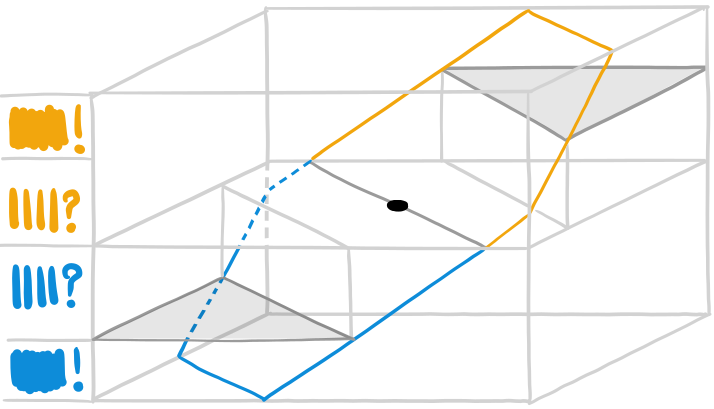
\includegraphics[width=0.49\textwidth]{./beach.png}%
  %  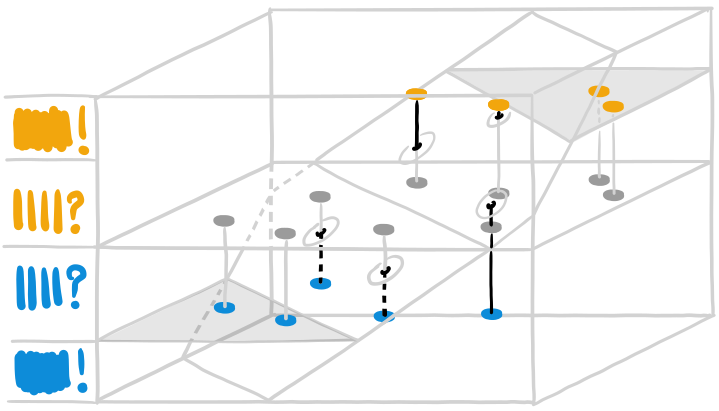
\includegraphics[width=0.85\textwidth]{./hinge-beach.png}%
  %  \caption{%
  %  \attnsam{caption}
  %  }
  %\end{figure}


